\section{Development Method} % (fold)
\label{sec:development}
% \meta{Describes BDD and why I choose it}

%intro
For a software project to be successful it is important to choose the right
development method. Two methods were considered for this project;
Behaviour-Driven Development (BDD) and Test-Driven Development (TDD).

BDD is an evolution of Test-Driven Development (TDD) which focus more on the
behaviour of the software instead of the structure (units). The problem with
TDD is that it focus on the internals of an object's implementation making
tests fails even when the behaviour of the code hasn't changed. In short TDD
tests what an object \textit{is} and BDD tests what an object
\textit{does}\cite{rspecbook}. Hence, BDD ensures business value is created and
works as intended, and TDD ensures that the code is correct but is blind to
whether it provides the intended business value.

BDD was chosen as the development method for this project due to it being an
improvement on TDD and allowing for rapid development without needing to
design the entire system up front. This agility makes it easier to spot
difficulties and caveats early the process, leaving more room to adapt. With
BDD (and TDD) the design is constantly evolving as more code is added and
former code is constantly reviewed and refactored. This form of design is
referred to as an emergent design. The following describes the BDD development
cycle and the tools used.

\subsection{Behaviour-Driven Development}
%intro
Behaviour-driven Development (BDD) revolves around writing specifications for
what a program is intended to do. This process is made up of an outer and an
inner loop. The outer loop concerns passing an acceptance test covering one
feature i.e.\ logging functionality. The inner loop concerns passing RSpec
behaviour specifications describing the behaviour of methods and objects.
Figure~\ref{bdd_cycle} depicts the BDD cycle.

\begin{figure}[htb]
  \centering
  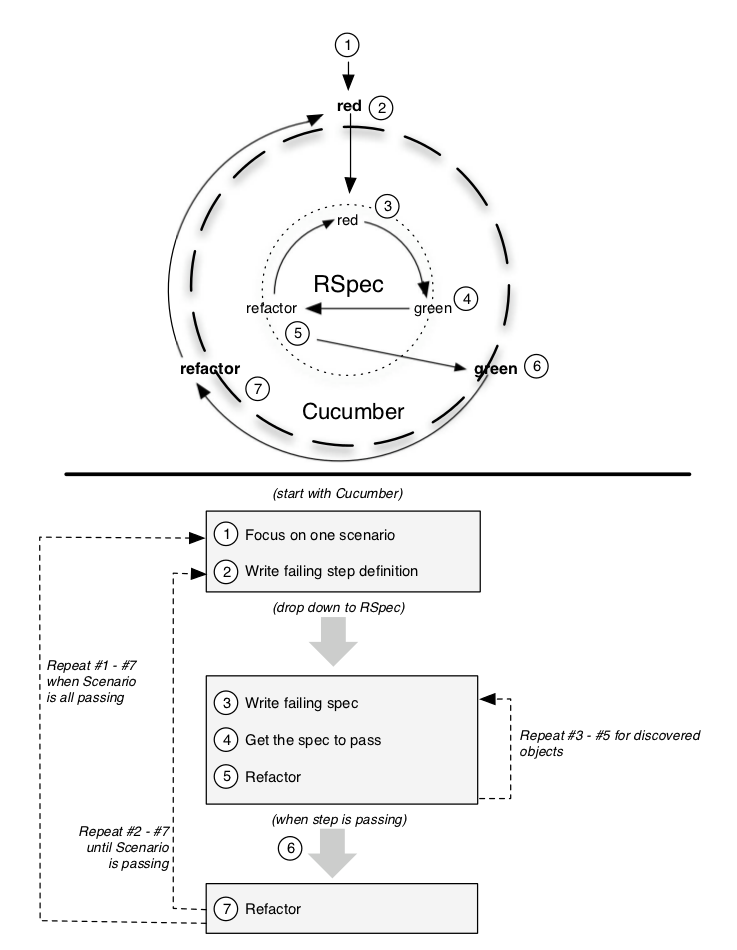
\includegraphics[width=0.9\textwidth]{img/bdd_cycle.png}
  \caption{The BDD development cycle\cite{rspecbook}}
  \label{bdd_cycle}
\end{figure}

%cycle, acceptance
At the beginning of the iteration an acceptance test is written and executing
it should reveal that the functionality is not yet implemented according to
it's requirements. Cucumber is a framework for writing acceptance tests in a
natural language as a set of steps in one or more scenarios.  An example
Cucumber acceptance test is included in Listing~\ref{cucumber_example}.

\bigskip
\begin{lstlisting}[label=cucumber_example,caption=Cucumber acceptance test example]
Feature: Logging
  As a webdeveloper
  I want to have logging of HTTP requests
  In order to debug errors or attacks on the webserver

  Scenario: Logging of HTTP requests
    Given the webserver is running
    When a user visits http://localhost/posts
    Then the log should contain "GET /posts"
    And the log should contain "SENT /posts SUCCESS"
\end{lstlisting}

The acceptance test covers the logging functionality of a webserver and tests it
by starting the webserver, making a request and then checking whether the log
contains the correct entry.  The first line names the feature covered by the
test. Lines 2 through 4 states the user of the feature, what it should do and
lastly why and what business value it creates. Line 6 states a specific
scenario, and often a feature has multiple scenarios and needs to test them
separately. Scenarios contains separate steps which defines either a
prerequisite (Given), an action (When) or a result (Then)\footnote{"And"
continues the previous step type}. The semantic of the steps are defined in a
set of step definitions written in plain Ruby.
Listing~\ref{step_definition_example} is a step definition of the step used on
line 9 in Listing~\ref{cucumber_example}.

\bigskip
\begin{lstlisting}[label=step_definition_example,caption=Cucumber step definition]
  Then /^the log should contain "([^"]*)"$/ do |entry|
    Server::log.should have(entry)
  end
\end{lstlisting}

The step definition checks whether the server log contains given entry using
RSpec. Steps are matched with regular expressions and \texttt{"([\^"]*)"}
matches the string "GET /posts" on line 9 in Listing~\ref{cucumber_example}.
Step definitions returns true if it passes and false if it didn't, and in the
case of a failure displays a detailed debug message.

%rspec -> red/green
RSpec is a BDD framework for Ruby used to write behaviour specifications
(specs). Specs are to BDD what unit tests are to TDD\@. Once the acceptance test is
written and run, steps will fail as they are not implemented (step 2 on
Figure~\ref{bdd_cycle}). Once implemented, steps might reveal application code
which is not yet available and therefore fail. In the example above, this error
could be caused by \texttt{Server} not having the method \texttt{log}. At this
point (point 3 on Figure~\ref{bdd_cycle}, an RSpec spec is needed to define the
behaviour of the \texttt{log} method. Listing~\ref{rspec_example} shows how such
a spec might look.

\bigskip
\begin{lstlisting}[label=rspec_example,caption=RSpec (spec) example]
describe Server do
  describe "#log" do
    it "should return an array" do
      Server.log << "Test string"
      Server.log.should.return(["Test string"])
    end
  end
end
\end{lstlisting}

Lines 1 and 2 in Listing~\ref{rspec_example} describes that we are specifying
the \texttt{log} method on the \texttt{Server} class. Line 3 describes the
intended behaviour of the \texttt{log} method; namely that it should return an
array. Then a test string is written to the log enabling the assertion that
calling the \texttt{log} method should return that exact string. The next step
in the BDD cycle is now to get the spec to pass (go from red to green) with
the simplest solution possible. In case of the example this would require
implementing the \texttt{log} method to return an array of log entries. Once
the spec passes, the code can be refactored if possible, and then the
developer moves on to the next failing step definition. This process is
continued until the acceptance test passes, meaning the feature is done.
